\chapter{Introduction}

\section{Introduction}
\acfp{LLM} were developed as a result of advancements in deep learning that allow them to read, understand, and create large amounts of natural language. The development of these \acp{LLM} has been directly linked to an architectural advancement known as the Transformer. This architecture allows for the ability to model sequences based upon their relevance (attention) and allowed  efficient training on larger than ever before data sets, in parallel \cite{vaswani2017attention}. With increases in both the amount of data available, computing power and model size, \acp{LLM} have achieved impressive results across a variety of tasks including question answering, generating summaries, coding, and extracting information \cite{brown2020language,kaplan2020scaling}. These capabilities have provided several opportunities for their use in various types of applications, however, with this come significant technical barriers for deployment \acp{LLM} due to the issues associated with memory usage during processing, processing speed/latency for real-time operations, reliance on other software packages, and ensuring reproducible results.

One technique used to improve both the utility and credibility of \acf{LLM} systems is called \acf{RAG}. The \ac{RAG} system takes advantage of a retrieval mechanism that pulls in relevant data from an outside body of documents, and then incorporates these retrieved data into the final input (i.e. model prompt), before generating an answer \cite{lewis2020rag,izacard2021leveraging}. Therefore, as opposed to answers being generated using only what is contained within the model's parameterized knowledge base, the answers are now supported by some form of evidence pulled directly from the outside world. In addition to supporting domain adaptation, \ac{RAG} can be done without additional model training or full weight-fine-tuning costs \cite{borgeaud2022retro}. 

At the same time as producing answers, \ac{RAG} systems aren't simply single-model systems. Document loading, chunking, embedding creation, indexing, retrieval (with optional reranking), prompt creation, answer creation, and log creation (i.e. logging results) occur during the operation of a typical \ac{RAG} system. Since each of these components can influence both the quality of the final answer created by the system and the amount of time it takes to execute the entire \ac{RAG} system, in addition to determining if an answer was generated, a successful \ac{RAG} project will also need to determine how different retrieval strategies impact latency, evidence quality, answer accuracy, and reproducibility.

This thesis also relates to \acf{HPC} as an appropriate area of deployment. Many \ac{HPC} systems have the characteristics of shared compute resources, job schedulers, execution environments that are based on containers, large-scale storage and scalable hardware in order to support high computational workloads \cite{dongarra2020hpcsurvey, kurtzer2017singularity,slurm2003}. The \ac{HPC} stage of this experiment builds upon the previous work done using notebooks and extends it to a much larger and more complex environment. Therefore, comparisons can be made with regard to timing behaviour when identical \ac{RAG} workflows are run in different environments.

\section{Motivation}

The primary purpose behind creating this project is to address the increasing demand for \acf{LLM} applications that use private domain-specific data or constantly evolving data. A single, self-contained language model will be able to generate coherent responses; however, it will likely lack immediate access to the specific documentation required to perform the desired function. Therefore, the model could potentially create responses that seem valid, yet would be unsupported by existing documented proof. This is where \ac{RAG} can help mitigate some of these limitations by allowing the system to search a previously established body of knowledge, retrieve relevant pieces of text, and pass these retrieved texts into the language model as supplementary input before generating an answer.

Although the idea of \ac{RAG} seems relatively simple, the performance and speed of a full \ac{RAG} solution heavily depends on how each piece of the solution is implemented. For example, building a very basic-in-memory retriever is easily accomplished and works well when working with smaller bodies of text. However, using a basic in-memory retriever will not provide the same level of persistence or deployment options as a vector database. For instance, while Milvus (a vector database) provides much better persistence options and a much more viable platform for working with large-scale retrieval requirements than an in-memory basic approach, it comes at an added expense through both set up costs and indexing costs. Although reranking can improve retrieval quality by reordering retrieved items, it adds another model to the pipeline and increases overall retrieval latency. Similarly, hybrid retrieval allows for the combination of semantic and keyword-based retrieval methods; however, it also adds increased complexity to the overall retrieval method.

This explains why this experimental comparison is conducted between in-memory retrieval, vector-database retrieval, vector-database retrieval with optimized chunking, dense retrieval with reranking, hybrid retrieval and finally hybrid retrieval with reranking (a combination of the latter two). Reproducible workflow is required because practical \ac{RAG} solutions comprise numerous service providers, models, notebooks, configuration files, result logs, evaluation scripts, and generated images for the results.

\section{Problem Definition}

The general problem addressed by this thesis is how to easily and practically test different versions of a \ac{RAG} pipeline under a deployment workflow that is fully reproducible. The primary issue is not whether \ac{RAG} will improve general language-model applications as other studies have shown \cite{lewis2020rag,izacard2021leveraging}, but instead, what effect do different retrieval and ranking strategies have on speed, the amount and quality of retrieved evidence, and the final quality of answers and how easy it is to reproduce these results.

A \ac{RAG} pipeline contains several components whose behaviour must be coordinated. Documents must be loaded into memory and split into chunks; embeddings must be generated; indexes or document stores must be created; candidate passages must be retrieved and finally, using the selected context, the language model must generate an answer. Weaknesses at any stage can reduce the usefulness of the final system. For example, while a fast retriever may return documents that are irrelevant to the user's query, these poorly chosen documents may lead to poor answers. Simultaneously, a re-ranking stage which may enhance the quality of the document choice may also result in significantly longer response times.

Therefore, the primary goal of this thesis is to study the implemented \ac{RAG} pipelines both as exploratory software deployment and experimental conditions. It compares their output using exactly the same input documents, scenario queries, models and logging approach. This creates a controlled framework from which to evaluate the trade-off between performance and output quality.

\section{Research Objectives and Scope}

The scope of this thesis is limited to retrieval-level \ac{RAG} experimentation and reproducible deployment workflow design. The local experiments provide the empirical comparison, while the \ac{HPC} workflow prepares for larger-scale execution.

The approach aims to use the same collections of documents, questions, open-source language and embedding models, as well as the same format for logging as much as possible throughout this thesis. This enables to measure the influence of different retrieval methods and deployment strategies independently. A baseline of behaviour using the developed notebooks during the local phase, is also established. During the \ac{HPC} phase, the same files and scenarios are executed to compare the results obtained in the local and \ac{HPC} environments within a common evaluation framework, with a focus on execution time.

To accomplish the objectives outlined in this thesis, the following five objectives will be met:

\begin{enumerate}

    \item \textbf{Provide the theoretical and practical foundations for \acp{LLM} and \ac{RAG} Systems.}\newline 
    The thesis discusses the background of the necessary concepts to distinguish between model-level techniques (e.g. fine-tuning, training from scratch, quantization, pruning, adaptation) and the retrieval-level techniques that are being assessed in this work. Additionally, it introduces the concepts of RAG, Dense \& Sparse Retrieval, Hybrid Retrieval, Reranking, Vector Databases, and HPC Deployment.
    
    \item \textbf{Implement and assess the effectiveness of various \ac{RAG} Retrieval Methods.}\newline   
    The thesis describes the six methods for retrieval implementations. Each of the implementations is evaluated using standard retrieval metrics, such as hit rate, precision, recall, and F1, along with quality metrics for answers, for instance manual correctness scores, ROUGE-L scores, BERTScores, and semantic similarity.
    
    \item \textbf{Determine the performance cost of the implemented \ac{RAG} pipelines.}\newline
    This objective describes the timing (in seconds) that is measured using the "notebooks" and shared CSV-style result logs, for each of the \ac{RAG}-pipelines built in this project. The metrics allow for a comparison of the costs of different processing methods such as in-memory-retrieval vs storage with a vector database, reranking retrieved candidates/passages from retrieval, sparse-dense retrieval combination, and varying the number of chunks.
    
    \item \textbf{Develop a workflow to compare local vs. \ac{HPC} execution.}\newline
    The local results that are initially collected, serve as a baseline for the \ac{HPC} extension of this work. The \ac{HPC} workflow is implemented using \ac{vLLM}-based model serving for generation, embeddings, and reranking where applicable.
    
    \item \textbf{Create a reproduciblee valuation framework.}\newline
    The thesis documents the software tools, execution procedures, scenario questions, logging fields, manual evaluation criteria, reproducibility scripts, and visualizations used during analysis.

\end{enumerate}

    This research limits its study to inference time \ac{LLM} and \ac{RAG} loads. This will enable the experiment to focus on retrieving quality answers as well as system performance. The scope does NOT include full model training or large-scale distributed training, model fine-tuning, model compression (quantization) or pruning, model distillation, and adapter based model optimization. These concepts have been referenced where necessary for a comparison in concept.

\section{Research Questions and Hypotheses}

The research questions are designed to remain within the experimental scope of the thesis. They focus on two measurable areas: the accuracy and answer quality of retrieval-level techniques, and the timing behaviour of the implemented workflows. The local experiments provide the first set of measurements, while the later \ac{HPC} experiments repeat the same workflow to evaluate portability and deployment behaviour.

\begin{itemize}
    \item {\bfseries RQ1:}
    \textbf{How do different retrieval techniques affect the retrieval-accuracy and answer-quality of the implemented \ac{RAG} pipelines?}\newline
    {\bf H1:} 
    Hybrid-retrieval will reach a better retrieval-coverage than dense-retrieval due to lexical-matching combined with semantic-similarity; Reranking will make sure that retrieved passages are ordered well and thus increase top-k precision, answer-grounded-ness, and answer-correctness. It is assumed that the combination of hybrid-retrieval and reranking will lead to the best retrieval-quality results particularly for those queries which need an understanding of their semantic interpretation as well as the correct wording. Another expected noticeable improvement is the tuned Vector database implementation.
    
    \item {\bfseries RQ2:}
    \textbf{What kinds of performance trade-offs are introduced through hybrid-retrieval and reranking?}\newline
    {\bfseries H2:} 
    The advantages at the level of retrieval are not cost-free in terms of execution-time. As a result, it is assumed that the retrieval-latency of the two basic (vector-database) pipelines will be lower than the one introduced by reranking and by hybrid-retrieval with reranking. Consequently, the best-performing pipeline concerning answer-quality might not be the fastest pipeline concerning end-to-end latency.
    
    \item {\bfseries RQ3:}
    \textbf{Which timing components dominate the execution cost of the implemented \ac{RAG} pipelines?}\newline
    {\bfseries H3:} 
    Generation time is anticipated to be the largest component of the overall processing time for almost all pipelines, while retrieval time is expected to grow in importance as more pipelines are added (reranked) or use a combination of both dense and sparse retrieval methods. The amount of indexing time will depend upon how the pipeline has been optimized for either in memory retrieval, a vector database, tuned chunking, or hybrid retrieval.
    
    \item {\bfseries RQ4:}
    \textbf{How does the same \ac{RAG} workflow behave, in terms of execution time, when moved from local to \ac{HPC} deployment?}\newline
    {\bfseries H4:} 
    The major differences are expected to occur with respect to timing behaviour when using the same six \ac{RAG} pipeline structures and the same five scenarios on both local and \ac{HPC} systems. On an \ac{HPC} system, it is expected that the overall time of a computation will be reduced significantly compared to a local environment; particularly where computations rely heavily upon data generation. However, there is no reason why all retrieval times would need to show improvement since vector database access, storage behaviour and service interactions can create overhead for short retrieval operations.
\end{itemize}

These hypotheses are designed to be compared and measured. They can be evaluated using retrieval-quality metrics, answer-quality rubrics, timing data, and labels showing whether the workflow was run locally or on HPC.

\section{Research Methodology Overview}

The methodology includes a literature study, a software implementation, controlled experiments, and an analysis of the qualitative output from these studies. Figure~\ref{fig:overall-thesis-workflow} summarizes this workflow.

\begin{figure}[htbp]
    \centering
    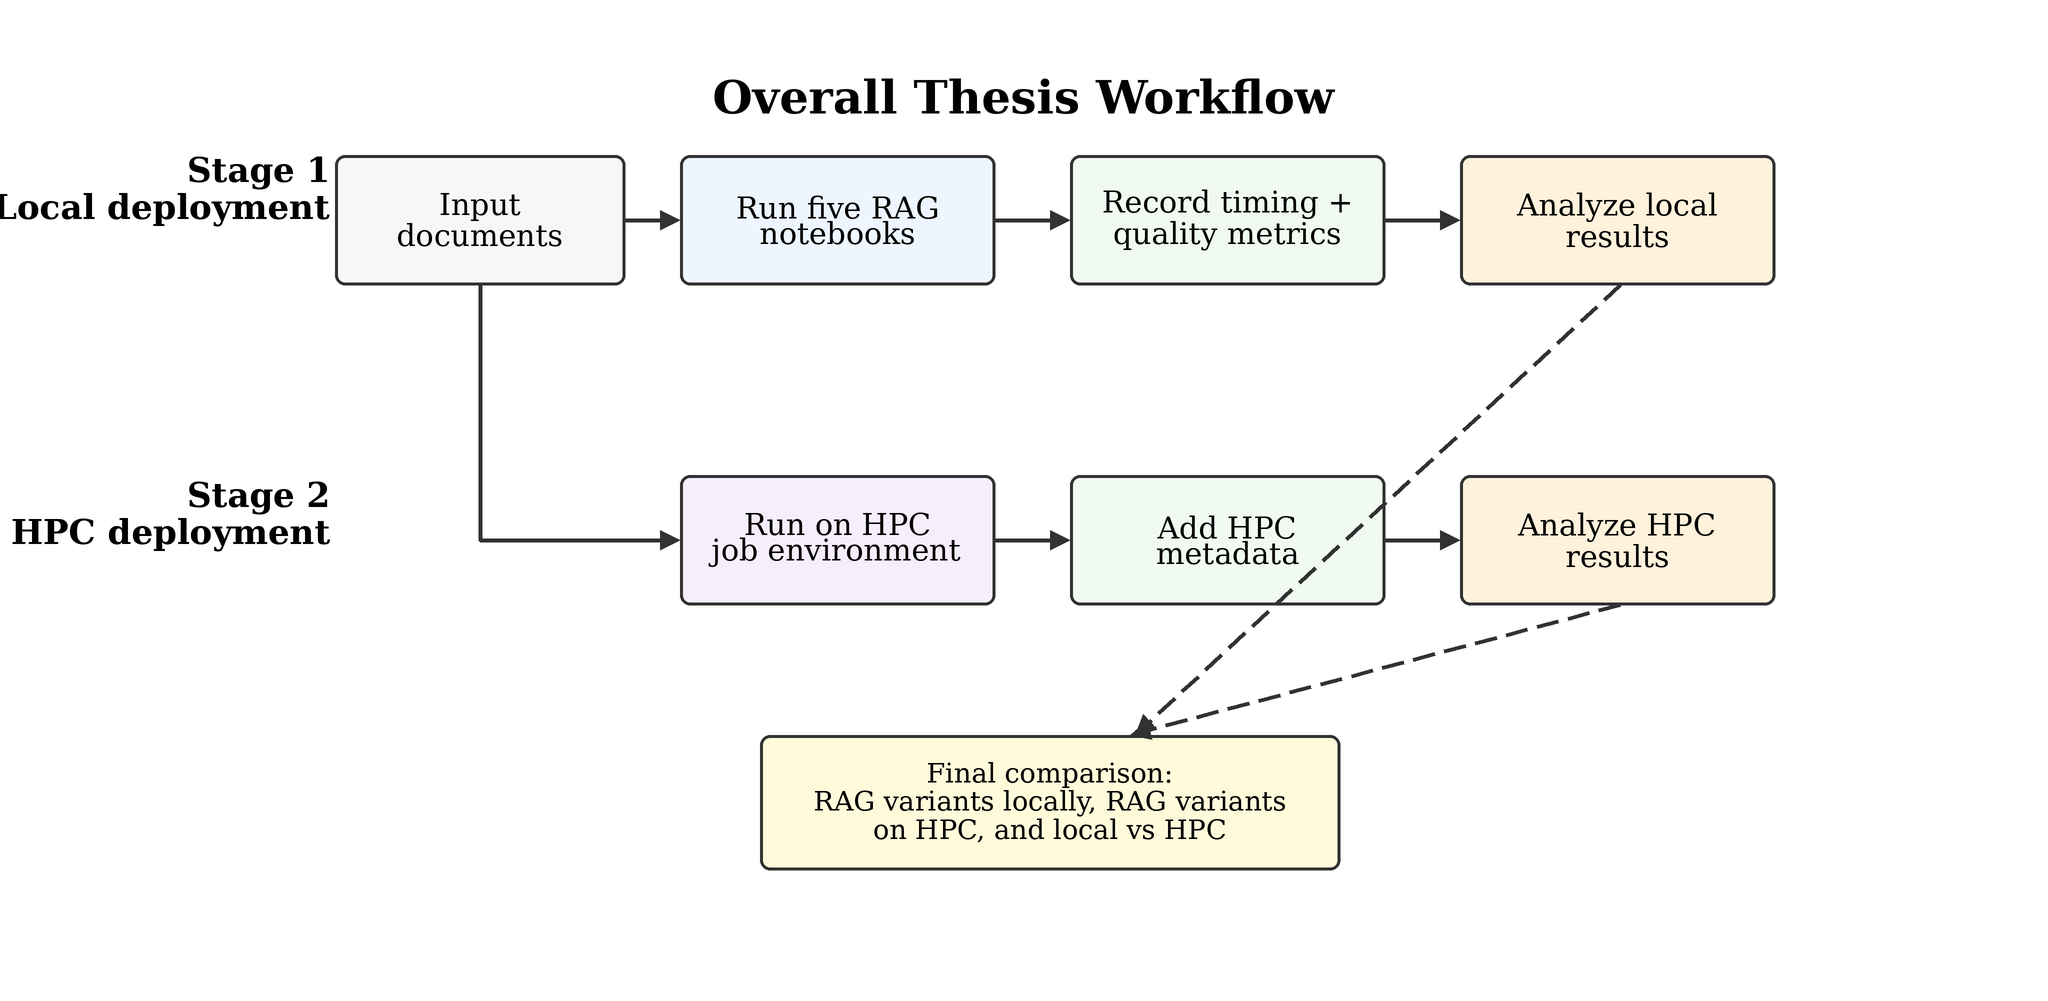
\includegraphics[width=\textwidth]{images/fig01_overall_thesis_workflow.png}
    \caption{Overall thesis workflow showing the local deployment stage, the later HPC deployment stage, and the final comparison between \ac{RAG} variants and execution environments.}
    \label{fig:overall-thesis-workflow}
\end{figure}

The first step develops the theoretical and technological basis for the studies. It reviews \acp{LLM}, transformer architectures, how prompts are generated, \ac{RAG} architectures, retrieval technologies, reranking, hybrid retrieval and \ac{HPC} as a technology for deploying systems. Step one (i) provides the vocabulary and context necessary to understand both the implementation (ii) and the results (iii).

Step two (ii) represents the implementation of the research pipeline; to organize the implementation into a series of six Jupyter notebooks. The content of each notebook includes; loading documents, preparing chunks, creating or connecting to the appropriate store (vector database), running query scenarios, generating answers and saving results.

The third step (iii) represents the evaluation process for each of the pipelines. To evaluate each pipeline, timing information is collected based on seconds. Indexing time, retrieval time and generation time are all included in this measurement. Additionally to collecting qualitative measurements of how well each pipeline performed, the source documents retrieved and the generated answers are also manually scored and analyzed utilizing deterministic metrics. The manual scores represent if the generated answer is correct or incorrect as determined by the evidence within the document corpus. Deterministic metrics utilized include retrieval hit, retrieval precision, retrieval recall, retrieval F1 score, ROUGE-L, BERTScore, semantic similarity and length of answer. Collecting both qualitative and quantitative measurements allows for an assessment of the trade-offs referenced in chapter~6.

\section{Expected Contributions}

\begin{enumerate}
    \item {\textbf{A reproducible local and \ac{HPC} workflow for evaluating \ac{RAG} pipelines.}}\newline
    The thesis presents a uniform execution environment to test the \ac{RAG} pipelines from the same document set, with the same evaluation questions, the same log formats, and the same evaluation workflow.
    
    \item {\textbf{An empirical comparison of six retrieval-level \ac{RAG} variants.}}\newline
    In this study, six retrieval-level \ac{RAG} variants are compared: in-memory retrieval, Milvus vector-database retrieval, tuned Milvus vector-database retrieval, dense retrieval with reranking, hybrid retrieval, and hybrid retrieval with reranking.
    
    \item {\textbf{An evaluation of quality and efficiency trade-offs.}}\newline
    This thesis evaluates the implemented pipelines through measurement of timing metrics, quality metrics for retrieval, and quality metrics for answers.
\end{enumerate}

Future directions include investigating larger-scale system-wide alternatives (e.g., caching mechanisms, batch processing capabilities, ability to execute multiple processes concurrently, measuring throughput of individual components, memory usage monitoring), additional datasets, and larger model families.

\section{Structure of the thesis}

The structure of the remainder of the thesis is described below.

\textit{\textbf{Chapter~2}} provides an overview of the theoretical foundations necessary for the development of the thesis. The chapter addresses; \acfp{LLM}, the Transformer architecture, model adaptation approaches, prompt engineering, \acf{RAG}, retrieval techniques, evaluation metrics and \acf{HPC} concepts.

\textit{\textbf{Chapter~3}} provides a review of existing literature referring to \acp{LLM} deployment and inference optimization, \ac{RAG} architectures and systems, retrieval techniques, and benchmarking methodologies.

\textit{\textbf{Chapter~4}} explains the methodology adopted. This includes a description of the research framework, the input data, the system architecture, the implemented \ac{RAG} pipelines, experimental parameters, performance metrics, answer-quality measures, and reproducibility procedures.

\textit{\textbf{Chapter~5}} describes how the experiments are set up and executed. This includes descriptions of the software environment, models/services, input corpus, notebook execution sequence, local and \ac{HPC} deployments, experiment scenarios, and result logging processes.

\textit{\textbf{Chapter~6}} reports and discusses the findings. The chapter will report and compare the results from each implemented pipeline by comparing them with respect to time-based metrics (timing); and retrieval/answer quality based metrics (retrieval quality and answer quality), as well as analyze the trade-off relationships between speed, retrieval quality, answer quality, and reproducibility.

\textit{\textbf{Chapter~7}} provides an overall summary of the conclusions drawn throughout the thesis, but also its limitations, and potential avenues for further research in areas such as additional datasets, larger model families, or other enhanced evaluation methodologies.

\section{Summary}

This Chapter introduced the motivations for this study, defined the research questions, provided an overview of the methodology used in this research, outlined what is intended as a contribution of this research, described how this study is organized, and identified the primary focus of this study which is to compare \ac{RAG} pipeline approaches at the retrieval level, provide reproducible local and \ac{HPC} execution workflow solutions, and to explore the trade-offs among retrieval quality, answer quality, performance and reproducibility. 
The next chapter will describe the theory necessary to develop a better understanding of \acp{LLM}, \acp{RAG}, various retrieval methods, evaluation metrics and HPC deployment concepts.
